\chapter{Zadanie 3}
\thispagestyle{chapterBeginStyle}
\label{rozdzial3}
\section{Opis problemu}
Zadanie polega na rozwiązaniu problemu minimalizacji czasu wykonywania zadań $J = \{1,2,...,n\}$ na $m$ maszynach.
Dla każdego zadania $i \in J$ dany jest czas potrzebny do wykonania $p_i$. 
Zbiór zadań jest uporządkowany za pomocą relacji poprzedzenia(zadanie 
$i$ może zostać wykonane po wykonaniu zadań $j_1,j_2$). 

\section{Rozwiązanie}
Do rozwiązania problemu stworzono program z parametrami: 
\begin{itemize}
    \item $p_i$ gdzie $i \in J$ czas wykonania zadania $i$;
    \item $r_i$ gdzie $i \in J$ zadania poprzedzające zadanie $i$;
    \item $m$ ilość maszyn 
\end{itemize}

Model rozwiązujący posiada:

\begin{itemize}
    \item Zmienną $x_{i,h,m}$ gdzie $i \in J, h \in Czas, m \in Maszyny$ opisującą czy zadanie $i$ uruchomi się w momencie $h$ na maszynie $m$;
    \item Zmienną $ms$ opisującą zakończenie ostatniego zadania;
    \item Ogarniczenie $\forall \substack{i \in J} \sum_{\substack{h \in Czas \\ m \in Maszyny}} x[i,h,m] == r_j$ 
    ogranicza uruchomienie każdego zadania tylko raz;
    \item Ogarniczenie $\forall \substack{h \in Czas \\ m \in Maszyny} \sum_{\substack{i \in J}} x[i,h,m] <= 1$ 
    ogranicza nakładanie się zadań w tym samym czasie na tej samej maszynie;
    \item Ogarniczenie $\forall \substack{i \in J} (\forall \substack{j \in r_i} \sum_{\substack{h \in Czas \\ m \in Maszyny}} x[j, h, m] * (h + p[j]) <= \sum_{\substack{h \in Czas \\ m \in Maszyny}} x[i, h, m] * h)$ ogranicza wykonywanie zadań po sobie;
    \item Ograniczenie $\forall \substack{h \in Czas \\ m \in Maszyny \\ i \in J} x[i, h, m] * (h + p[i]) <= ms$ ograniczającą zakończenie się ostatniego zadania;
    \item Funkcję celu $min \rightarrow ms$.
\end{itemize}


\section{Wyniki}

Rozwiązanie przykładu podanego w zadaniu \ref{zadanie3}. Rozwiązanie zostało zaprezentowane w tabeli \ref{tabela_zad3}
\begin{figure}[h]
    \centering
    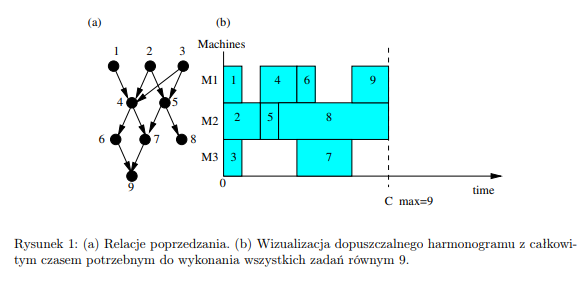
\includegraphics[scale=1.0]{zadanie3.png}
    \caption{Dane i rozwiązanie}
    \label{zadanie3}
\end{figure}

\begin{table}[ht]
    \begin{center}
        \begin{tabular}{| c | c | c | c |} 
            \hline
            \rowcolor{lgray}
            \backslashbox{czas}{maszyna} & 1 & 2 & 3 \\
            \hline
            1  &  1 & - & 2 \\
            2  &  - & 3 & 2 \\
            3  &  - & 5 & 4 \\
            4  &  - & 8 & 4 \\
            5  &  - & 8 & 7 \\
            6  &  - & 8 & 7 \\
            7  &  6 & 8 & 7 \\
            8  &  - & 8 & 9 \\
            9  &  - & 8 & 9 \\
            \hline
        \end{tabular}
        \caption{Wyniki rozwiązania}
        \label{tabela_zad3}
    \end{center}
\end{table}